\subsection{Procesamiento}

Se tomaron en cuenta restricciones sobre el brazo robótico a controlar y los servomotores posicionales a los que se envían las instrucciones.

El tipo de brazo robótico a controlar tiene un diseño antropomórfico, lo que significa que se compone de articulaciones unidas entre sí; además es de dos grados de libertad, lo que implica que tiene exactamente dos articulaciones. Como lo que interesa es controlar la posición (y no la orientación), se restringió la cantidad de grados de libertad del brazo robótico a uno en cada unión; esto significa que en la unión de la base existe un grado de libertad, y el otro grado de libertad se encuentra en la unión entre la primera y la segunda articulación. Además, ambos grados de libertad se mueven de arriba hacia abajo. Para alcanzar todas las posiciones posibles en el espacio, existe un grado de libertad adicional en la base que rota el brazo robótico alrededor de su eje. La Figura \ref{fig:tipobrazo} muestra un ejemplo de un brazo robótico que cumple con estas restricciones.

\begin{figure}[htb]
	\centering
	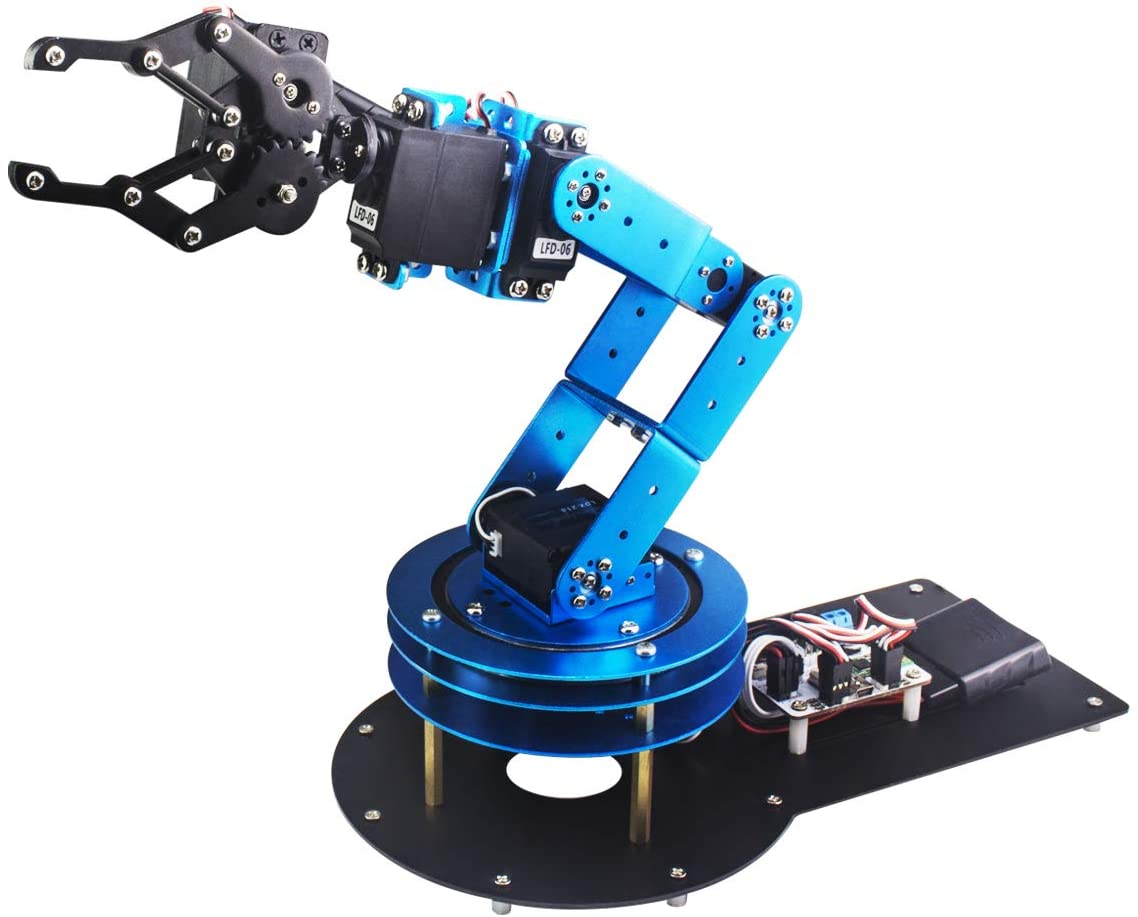
\includegraphics[scale=0.2]{tipobrazo.jpg}
	\caption{Brazo robótico de 2 DoF que cumple las restricciones impuestas}
	\label{fig:tipobrazo}
\end{figure}

El brazo robótico tiene la base en el suelo; esto significa que se puede mover dentro y en el contorno curvo de la mitad de una esfera con centro en la base del robot y de radio igual a la longitud del robot; debido a que la ortesis utilizada para localizar la posición tiene 42 cm de largo, ésta es la máxima longitud del brazo para el sistema. Los servomotores posicionales solo pueden moverse en ángulos discretos, en particular, enteros. Esto significa que pueden alcanzar 180 posiciones. Además, muchas posiciones finales son lo suficientemente cercanas entre sí como para considerar que se aproximan a la misma posición.  Para determinar la proximidad de las posiciones, se aplicó el siguiente criterio con distancia Euclidiana entre dos posiciones. Si $P_1 = (x_1, y_1, z_1)$ es un punto en el espacio tal que sus coordenadas son valores enteros y $P_2 = (x_2, y_2, z_2)$ es cualquier otro punto:

\begin{equation}
	d(P_1, P_2) = \sqrt{(x_2 - x_1)^2 + (y_2 - y_1)^2 + (z_2 - z_1)^2} <= \frac{\sqrt{2}}{2} \approx 0.707
\end{equation}

De este modo, se considera que aquellos puntos que tienen a lo más 0,707 cm de distancia euclidiana entre ellos llegan a la misma posición. Para el caso en el que una de las coordenadas del punto $P_2$ sea entera, su distancia euclidiana al punto $P_1$ más cercano será menor que o igual a 0,5 cm, de modo que el criterio se reducirá a ese valor máximo. Si las posiciones alcanzables son como el punto $P_1$ antes descrito, esto significa que las posiciones alcanzables dentro del volumen de la semiesfera donde se puede mover el brazo robótico se reducen, lo que optimiza la determinación de la posición final. Note que la imprecisión es a lo más de 0.707 cm. 

Podemos notar que muchas posiciones pueden ser alcanzadas por un brazo robótico de una determinada longitud de articulaciones con más de una combinación de ángulos; por ejemplo, si la base tiene 0°, y ambas articulaciones tienen 90° y 0°, respectivamente, se alcanza la misma posición que si la base tiene 180°, y ambas articulaciones tienen 90° y 180°, respectivamente. En particular, si colocamos un plano paralelo al diámetro de la semiesfera que la atraviese, podemos notar las configuraciones ``espejo'' que alcanzan la misma posición. De modo que se restringió el rango de movilidad de las articulaciones de 0 a 90° para reducir aún más el espacio de búsqueda; la base se mantuvo de 0 a 360°. 

Si consideramos además que las longitudes de los brazos varían, esto significa que cada punto $P_1$ puede ser alcanzado por varias combinaciones distintas de longitudes de articulaciones y ángulos. Esto se aprovechó para reducir la cantidad de operaciones realizadas para determinar la cinemática inversa; dada una posición $P = (x,y,z)$ con las características de $P_1$, existe un conjunto de combinaciones de longitudes de articulaciones y ángulos de inclinación que alcanzan dicha posición (aplicando el criterio de la distancia euclidiana). Se consideró que estaban asociadas a dicha posición. Las longitudes $L_1$ y $L_2$ de las articulaciones se redondearon a valores enteros, considerando el criterio de que dos longitudes cuya diferencia es a lo más de 0.5 cm se acercan a posiciones muy próximas entre sí utilizando los mismos ángulos. Asimismo para longitudes más pequeñas, dos ángulos de inclinación o más que estén muy próximos entre sí pueden hacer que una articulación llegue a una misma posición, de modo que se considera que, para determinado rango de longitudes, los saltos en los valores de los ángulos sean mayores que 1. Se eligió dividir el rango de la longitud del brazo en 6 rangos; el primero, de 1 cm a 7 cm, tuvo saltos de 6°, el segundo, de 8 cm a 14 cm tuvo saltos de 5°, mientras que el tercero, de 15 cm a 21 cm tuvo saltos de 4°; de este modo, sucesivamente hasta el último rango, que va de 36 cm a 42 cm tuvo saltos de 1° por cada posición considerada.

Esto nos da las siguientes restricciones para generar el conjunto de datos de entrenamiento:

\begin{itemize}
	
	\item $ 1 \leq L_1, L_2 \leq 42; L_1, L_2 \in \mathbb{N}$ 
	
	\item $\alpha_1, \alpha_2, \alpha_3 \in \mathbb{Z}$; El ángulo de la base es $ 0 \leq \alpha_1 \leq 360$, mientras que los ángulos de inclinación de las articulaciones son $ 0 \leq \alpha_2, \alpha_3 \leq 90$
	
	\item Desarrollar e implementar una interfaz gráfica de usuario por medio del framework Qt para visualizar en una pantalla táctil de 7 pulgadas la cinemática inversa del brazo robótico a controlar.
	
	\item Implementar la comunicación entre el software SettDev y el PLC Kaab utilizando el módulo para el control de servomotores instalado en el PLC para enviar los ángulos de inclinación al controlador y reproducir los ángulos de inclinación en los servomotores posicionales.
	
\end{itemize}